\documentclass[12pt, letterpaper, titlepage]{article}
\usepackage[letterpaper,top=2cm,bottom=2cm,left=3cm,right=3cm,marginparwidth=1.75cm]{geometry}
\SetSymbolFont{letters}{normal}{OML}{txmi}{m}{it}
\DeclareSymbolFont{matha}{OML}{txmi}{m}{it}% txfonts
\DeclareMathSymbol{l}{\mathord}{matha}{21}
\usepackage[T1,T2A]{fontenc}
\usepackage[russian]{babel}
\usepackage[utf8]{inputenc}
\usepackage{amsmath}
\usepackage{parskip}
\usepackage{svg}
\usepackage{array}
\usepackage{float}
\usepackage{caption}
\usepackage[small]{titlesec}
\usepackage{amssymb}
\usepackage{listings}
\usepackage{xcolor}
\let\oldemptyset\emptyset
\let\emptyset\varnothing
\clubpenalty=10000 
\widowpenalty=10000
\title{"Курсовая работа по дискретной математике"}
\author{Иван Кочкожаров, студент группы М8О-108Б-22}
\begin{document}
\begin{titlepage}

    \thispagestyle{empty}
    
    \centerline{Министерство образования и науки РФ}
    \centerline{ФЕДЕРАЛЬНОЕ ГОСУДАРСТВЕННОЕ БЮДЖЕТНОЕ}
    \centerline{ОБРАЗОВАТЕЛЬНОЕ
    УЧРЕЖДЕНИЕ ВЫСШЕГО ОБРАЗОВАНИЯ}
    \centerline{<<МОСКОВСКИЙ АВИАЦИОННЫЙ ИНСТИТУТ}
    \centerline{(НАЦИОНАЛЬНЫЙ ИССЛЕДОВАТЕЛЬСКИЙ УНИВЕРСИТЕТ)>>}
    
    \vfill
    
    \centerline{\Huge{Курсовая работа}}
    \centerline{\large{по дисциплине}}
    \centerline{\Huge{<<Дискретная математика>>}}
    
    \vfill
    
    Студент группы М8О-108Б-22 \hfill Кочкожаров И.В.
    
    Преподаватель \hfill Осипова В.А.
    
    \vfill
    
    \centerline{Москва, 2023}
    \clearpage
\end{titlepage}
\setcounter{page}{2}
\textbf{1.} Определить для орграфа, заданного матрицей смежности $A$ =
$
    \begin{pmatrix}
        0 & 1 & 0 & 1 \\
        0 & 0 & 0 & 1 \\
        1 & 1 & 0 & 1 \\
        0 & 0 & 0 & 0 \\
    \end{pmatrix}
$
\begin{itemize}
    \item[a)] матрицу односторонней связности;
    \item[б)] матрицу сильной связности;
    \item[в)] компоненты сильной связности;
    \item[г)] матрицу контуров.
\end{itemize}
\underline{\textbf{Решение.}}

\emph{Изображение графа:}
\begin{figure}[H]\centering\includesvg[scale=0.33]{graphs/graph1}\caption{Граф $G$}\end{figure}
\emph{Матрица односторнней связности:}
\begin{equation*}
    A = A(D) =
    \begin{tabular}{ | c | c | c | c | c | c | }
        \hline
                & $v_{1}$ & $v_{2}$ & $v_{3}$ & $v_{4}$ \\
        \hline
        $v_{1}$ & 0       & 1       & 0       & 1       \\
        \hline
        $v_{2}$ & 0       & 0       & 0       & 1       \\
        \hline
        $v_{3}$ & 1       & 1       & 0       & 1       \\
        \hline
        $v_{4}$ & 0       & 0       & 0       & 0       \\
        \hline
    \end{tabular}.
\end{equation*}
$
    A^{2} =
    \begin{pmatrix}
        0 & 1 & 0 & 1 \\
        0 & 0 & 0 & 1 \\
        1 & 1 & 0 & 1 \\
        0 & 0 & 0 & 0 \\
    \end{pmatrix}
    \begin{pmatrix}
        0 & 1 & 0 & 1 \\
        0 & 0 & 0 & 1 \\
        1 & 1 & 0 & 1 \\
        0 & 0 & 0 & 0 \\
    \end{pmatrix}
    =
    \begin{pmatrix}
        0 & 0 & 0 & 1 \\
        0 & 0 & 0 & 0 \\
        0 & 1 & 0 & 1 \\
        0 & 0 & 0 & 0 \\
    \end{pmatrix}.
$\\
$
    A^{3} = A \cdot A^{2} =
    \begin{pmatrix}
        0 & 1 & 0 & 1 \\
        0 & 0 & 0 & 1 \\
        1 & 1 & 0 & 1 \\
        0 & 0 & 0 & 0 \\
    \end{pmatrix}
    \begin{pmatrix}
        0 & 0 & 0 & 1 \\
        0 & 0 & 0 & 0 \\
        0 & 1 & 0 & 1 \\
        0 & 0 & 0 & 0 \\
    \end{pmatrix}
    =
    \begin{pmatrix}
        0 & 0 & 0 & 0 \\
        0 & 0 & 0 & 0 \\
        0 & 0 & 0 & 1 \\
        0 & 0 & 0 & 0 \\
    \end{pmatrix}.
$
\begin{equation*}
    \begin{split}
        T(D) = E \lor A \lor A^{2} \lor A^{3} =
        \begin{pmatrix}
            1 & 0 & 0 & 0 \\
            0 & 1 & 0 & 0 \\
            0 & 0 & 1 & 0 \\
            0 & 0 & 0 & 1 \\
        \end{pmatrix}
        \lor
        \begin{pmatrix}
            0 & 1 & 0 & 1 \\
            0 & 0 & 0 & 1 \\
            1 & 1 & 0 & 1 \\
            0 & 0 & 0 & 0 \\
        \end{pmatrix}
        \lor &
        \begin{pmatrix}
            0 & 0 & 0 & 1 \\
            0 & 0 & 0 & 0 \\
            0 & 1 & 0 & 1 \\
            0 & 0 & 0 & 0 \\
        \end{pmatrix}
        \lor\\
        \lor
        \begin{pmatrix}
            0 & 0 & 0 & 0 \\
            0 & 0 & 0 & 0 \\
            0 & 0 & 0 & 1 \\
            0 & 0 & 0 & 0 \\
        \end{pmatrix}
        =
        \begin{pmatrix}
            1 & 1 & 0 & 1 \\
            0 & 1 & 0 & 1 \\
            1 & 1 & 1 & 1 \\
            0 & 0 & 0 & 1 \\
        \end{pmatrix}.
    \end{split}
\end{equation*}
\emph{Матрица двусторонней связности:}
\begin{equation*}
    S(D) = T(D) \& [T(D)]^\mathrm{T} =
    \begin{pmatrix}
        1 & 1 & 0 & 1 \\
        0 & 1 & 0 & 1 \\
        1 & 1 & 1 & 1 \\
        0 & 0 & 0 & 1 \\
    \end{pmatrix}
    \&
    \begin{pmatrix}
        1 & 0 & 1 & 0 \\
        1 & 1 & 1 & 0 \\
        0 & 0 & 1 & 0 \\
        1 & 1 & 1 & 1 \\
    \end{pmatrix}
    =
    \begin{pmatrix}
        1 & 0 & 0 & 0 \\
        0 & 1 & 0 & 0 \\
        0 & 0 & 1 & 0 \\
        0 & 0 & 0 & 1 \\
    \end{pmatrix}.
\end{equation*}
$S(D)=E\Rightarrow$ в графе $D$ нет контуров.

\emph{Компонентны сильной связности:}
\begin{equation*}
    S_2(D) = S(D) =
    \begin{tabular}{ | c | c | c | c | c | c | }
        \hline
                & $v_{1}$ & $v_{2}$ & $v_{3}$ & $v_{4}$ \\
        \hline
        $v_{1}$ & 1       & 0       & 0       & 0       \\
        \hline
        $v_{2}$ & 0       & 1       & 0       & 0       \\
        \hline
        $v_{3}$ & 0       & 0       & 1       & 0       \\
        \hline
        $v_{4}$ & 0       & 0       & 0       & 1       \\
        \hline
    \end{tabular}
\end{equation*}
$D_1=(V_1,X_1), V_1=\{v_1\}$

$A(D_1)=$
\begin{tabular}{|c|c|}
    \hline
            & $v_{1}$ \\
    \hline
    $v_{1}$ & 0       \\
    \hline
\end{tabular}\hspace{1cm}$D_1:$\hspace{1cm}
\includesvg[scale=0.09]{graphs/cfc1}

\begin{equation*}
    S_2(D) =
    \begin{tabular}{ | c | c | c | c |  }
        \hline
                & $v_{2}$ & $v_{3}$ & $v_{4}$ \\
        \hline
        $v_{2}$ & 1       & 0       & 0       \\
        \hline
        $v_{3}$ & 0       & 1       & 0       \\
        \hline
        $v_{4}$ & 0       & 0       & 1       \\
        \hline
    \end{tabular}
\end{equation*}
$D_2=(V_2,X_2), V_2=\{v_2\}$

$A(D_2)=$
\begin{tabular}{|c|c|}
    \hline
            & $v_{2}$ \\
    \hline
    $v_{2}$ & 0       \\
    \hline
\end{tabular}\hspace{1cm}$D_2:$\hspace{1cm}
\includesvg[scale=0.09]{graphs/cfc2}

\begin{equation*}
    S_3(D) =
    \begin{tabular}{ | c | c | c |  }
        \hline
                & $v_{3}$ & $v_{4}$ \\
        \hline
        $v_{3}$ & 1       & 0       \\
        \hline
        $v_{4}$ & 0       & 1       \\
        \hline
    \end{tabular}
\end{equation*}
$D_3=(V_3,X_3), V_3=\{v_3\}$

$A(D_3)=$
\begin{tabular}{|c|c|}
    \hline
            & $v_{3}$ \\
    \hline
    $v_{3}$ & 0       \\
    \hline
\end{tabular}\hspace{1cm}$D_3:$\hspace{1cm}
\includesvg[scale=0.09]{graphs/cfc3}

\begin{equation*}
    S_4(D) =
    \begin{tabular}{ | c | c | }
        \hline
                & $v_{4}$ \\
        \hline
        $v_{4}$ & 1       \\
        \hline
    \end{tabular}
\end{equation*}
$D_4=(V_4,X_4), V_4=\{v_4\}$

$A(D_4)=$
\begin{tabular}{|c|c|}
    \hline
            & $v_{4}$ \\
    \hline
    $v_{4}$ & 0       \\
    \hline
\end{tabular}\hspace{1cm}$D_4:$\hspace{1cm}
\includesvg[scale=0.09]{graphs/cfc4}

\emph{Матрица контуров:}
\begin{equation*}
    K(D)=A(D) \& S(D) =
    \begin{pmatrix}
        0 & 1 & 0 & 1 \\
        0 & 0 & 0 & 1 \\
        1 & 1 & 0 & 1 \\
        0 & 0 & 0 & 0 \\
    \end{pmatrix}
    \begin{pmatrix}
        1 & 0 & 0 & 0 \\
        0 & 1 & 0 & 0 \\
        0 & 0 & 1 & 0 \\
        0 & 0 & 0 & 1 \\
    \end{pmatrix}
    =
    \begin{pmatrix}
        0 & 0 & 0 & 0 \\
        0 & 0 & 0 & 0 \\
        0 & 0 & 0 & 0 \\
        0 & 0 & 0 & 0 \\
    \end{pmatrix}
\end{equation*}

\textbf{2.} Используя алгоритм Терри, определить замкнутый маршрут, проходящий ровно по два раза
(по одному в каждом направлении) через каждое ребро графа.
\begin{figure}[H]\centering\includesvg[scale=0.65]{graphs/init_terry}\caption{Граф $G$}\end{figure}
\underline{\textbf{Решение.}}

Для решения этой задачи действуем в соответствии с алгоритмом Тэрри.
Для реализации алгоритма помечаем первые заходящие в вершины ребра крестиками, которые наносим на
ребрах ближе к той вершине в которую в первый
раз заходим, а также указываем направления прохождения ребер и последовательность
прохождения ребер. Алгоритм дает следующий возможный маршрут:
\begin{equation*}
    v_1v_2v_3v_5v_4v_3v_4v_2v_4v_1v_4v_5v_3v_2v_1
\end{equation*}
\begin{figure}[H]\centering\includesvg[scale=1]{graphs/terry}\caption{Визуализация алгоритма Терри}\end{figure}
\iffalse
    \textbf{3.} Используя алгоритм “фронта волны”, найти все минимальные пути из первой вершины в
    последнюю орграфа, заданного матрицей смежности
    \begin{equation*}
        A =
        \begin{pmatrix}
            0 & 0 & 1 & 0 & 0 & 1 & 0 & 0 \\
            1 & 0 & 1 & 1 & 1 & 1 & 0 & 0 \\
            1 & 0 & 0 & 0 & 0 & 1 & 0 & 0 \\
            1 & 1 & 1 & 0 & 0 & 1 & 0 & 0 \\
            1 & 1 & 1 & 1 & 0 & 0 & 1 & 1 \\
            0 & 0 & 1 & 1 & 0 & 0 & 0 & 0 \\
            1 & 0 & 1 & 1 & 1 & 1 & 1 & 0 \\
            1 & 0 & 1 & 1 & 0 & 0 & 1 & 0 \\
        \end{pmatrix}.
    \end{equation*}
\fi
\textbf{3.} Орграф $D=(V,X)$, где $V = \{v_1, \dots, v_{10}\}$ задан матрицей
смежности $A(D)$. Найти все минимальные пути $v_1$ в $v_{8}$.
\begin{equation*}
    A = A(D) =
    \begin{tabular}{ | c | c | c | c | c | c | c | c | c |}
        \hline
              & $v_1$ & $v_2$ & $v_3$ & $v_4$ & $v_5$ & $v_6$ & $v_7$ & $v_8$ \\
        \hline
        $v_1$ & 0     & 0     & 1     & 0     & 0     & 1     & 0     & 0     \\
        \hline
        $v_2$ & 1     & 0     & 1     & 1     & 1     & 1     & 0     & 0     \\
        \hline
        $v_3$ & 1     & 0     & 0     & 0     & 0     & 1     & 0     & 0     \\
        \hline
        $v_4$ & 1     & 1     & 1     & 0     & 0     & 1     & 0     & 0     \\
        \hline
        $v_5$ & 1     & 1     & 1     & 1     & 0     & 0     & 1     & 1     \\
        \hline
        $v_6$ & 0     & 0     & 1     & 1     & 0     & 0     & 0     & 0     \\
        \hline
        $v_7$ & 1     & 0     & 1     & 1     & 1     & 1     & 1     & 0     \\
        \hline
        $v_8$ & 1     & 0     & 1     & 1     & 0     & 0     & 1     & 0     \\
        \hline
    \end{tabular}.
\end{equation*}
\underline{\textbf{Решение.}}

Действуя согласно алгоритму фронта волны, последовательно определяем:

$FW_0(v_1)=\{v_1\}, FW_1(v_1)=D(v_1)=\{v_3,v_6\},$\\
$FW_2(v_1)=D(FW_1(v_1)) \setminus (FW_0(v_1) \cup FW_1(v_1))=D(\{v_3,v_6\}) \setminus \{v_1,v_3,v_6\}=$\\
$=\{v_1,v_3,v_4,v_6\} \setminus \{v_1,v_3,v_6\}=\{v_4\}$\\
$FW_3(v_1)=D(FW_2(v_1)) \setminus (FW_0(v_1)\cup FW_1(v_1)\cup FW_2(v_1))=\{v_1,v_2,v_3,v_6\} \setminus$\\
$\setminus \{v_1,v_3,v_4,v_6\}=\{v_2\}$\\
$FW_4(v_1)=D(FW_3(v_1)) \setminus (FW_0(v_1)\cup FW_1(v_1)\cup FW_2(v_1)\cup FW_3(v_1))=$\\
$=\{v_1,v_3,v_4,v_5,v_6\} \setminus \{v_1,v_2,v_3,v_4,v_6\}=\{v_5\}$\\
$FW_5(v_1)=D(FW_4(v_1)) \setminus (FW_0(v_1)\cup FW_1(v_1)\cup FW_2(v_1)\cup FW_3(v_1)\cup FW_4(v_1))=$\\
$\{v_1,v_2,v_3,v_4,v_7,v_8\}\setminus \{v_1,v_2,v_3,v_4,v_5,v_6\}=\{v_7,v_8\}$

Таким образом, $v_8 \in FW_5(v_1)$, а следовательно, согласно алгоритму фронта волны существует минимальный
путь в орграфе $D$ из $v_1$ в $v_8$ длины 5. Найдём все эти пути.
\begin{figure}[H]\centering\includesvg[scale=0.45]{graphs/fw1}\caption{Граф D'}\end{figure}
На рисунке 4 изображен подграф $D'$ орграфа $D$, на котором последовательно изображены множества
$FW_k(v_1), k=1,2,3,4,5$, а так же  дуги вида $(v, v')$, где для некоторого $k \in \{0,1,2,3,4\},
    v \in FW_k(v_1), v' \in FW_{k+1}(v_1)$, т.е. исходящие из вершин некоторого $k$-го фронта волны и
заходящие в вершины следующего $(k+1)$-го фронта волны.

Используя изображение $D'$ нетрудно выделить все минимальные пути из $v_1$ в $v_8$
в орграфе $D$. При этом, следуя алгоритму фронта волны, находим эти минимальные пути, используя орграф $D'$
но двигаясь в $D'$ в обратной последовательности (т.е. не из $v1$ в $v_8$ а наоборот, из $v_8$
в $v_1$ ). Используя рисунок 4, получаем, что в любом минимальном пути из $v_1$ в $v_8$
соблюдается следующая последовательность вершин. Вершиной, предшествующей
вершине $v_8$ может быть $v_5$. Вершиной, предшествующей вершине $5$
может быть $v_2$. Вершиной, предшествующей вершине $v_2$ – вершина $v_4$.
Вершиной, предшествующей вершине $v_4$ – любая из вершин $v_3,v_6$.
Вершиной, предшествующей вершинам $v_3$ и $v_6$ может быть только $v_1$. Этими условиями однозначно определяется множество
минимальных путей из $v_1$ в $v_8$ которое компактно изображено на рисунке 5. На этом
рисунке изображены все вершины, входящие в минимальные пути $v_1$ в $v_8$ Для каждой
из промежуточных вершин $v$ показано множество вершин, которые могут ей
предшествовать, а также соответствующие дуги (исходящие из вершин, предшествующих $v$
и заходящие в $v$). Из рисунка 5 видно, что всего существует два минимальных пути из $v_1$ в
$v_8$: $v_1v_3v_4v_2v_5v_8$, $v_1v_6v_4v_2v_5v_8$.
\begin{figure}[H]\centering\includesvg[scale=0.5]{graphs/fw2}\caption{Граф минимальных путей}\end{figure}
\newpage
\textbf{4.} Нагруженный орграф $D$ задан матрицей длин дуг $C(D)$. Найти минимальные пути из $v_1$ во все достижимые вершины.
\[
    C(D)=
    \begin{pmatrix}
        \infty & 4      & \infty & \infty & 5      & \infty & \infty & \infty \\
        5      & \infty & 7      & 10     & 2      & \infty & \infty & \infty \\
        \infty & \infty & \infty & 2      & \infty & 2      & \infty & \infty \\
        6      & \infty & \infty & \infty & \infty & \infty & 3      & 5      \\
        3      & 2      & \infty & \infty & \infty & 3      & 11     & \infty \\
        4      & \infty & 2      & \infty & \infty & \infty & 7      & \infty \\
        8      & \infty & \infty & 3      & \infty & \infty & \infty & 3      \\
        \infty & \infty & \infty & \infty & 17     & \infty & \infty & \infty \\
    \end{pmatrix}
\]

\underline{\textbf{Решение.}}

Воспользуемся алгоритмом Форда. Сначала определим таблицу величин $l_{i}^{(i)}, i=1,2,\dots,n-1$, где $n=8$
\begin{center}
    \begin{tabular}{ | c | c | c | c | c | c | c | c | c | c |c |c |c |c |c |c |c |c |}
        \hline
        \rule{0pt}{13pt} & $v_1$      & $v_2$      & $v_3$      & $v_4$       & $v_5$       & $v_6$       & $v_7$     & $v_8$     &
                         & $l^{(0)}$  & $l^{(1)}$  & $l^{(2)}$  & $l^{(3)}$   & $l^{(4)}$   & $l^{(5)}$   & $l^{(6)}$ & $l^{(7)}$   \\
        \hline
        $v_1$            & $\infty$   & 4          & $\infty$   & $\infty$    & 5           & $\infty$    & $\infty$  & $\infty$  &
                         & \textbf{0} & 0          & 0          & 0           & 0           & 0           & 0         & 0           \\
        \hline
        $v_2$            & 5          & $\infty$   & 7          & 10          & 2           & $\infty$    & $\infty$  & $\infty$  &
                         & $\infty$   & 4          & 4          & 4           & 4           & 4           & 4         & 4           \\
        \hline
        $v_3$            & $\infty$   & $\infty$   & $\infty$   & 2           & $\infty$    & 2           & $\infty$  & $\infty$  &
                         & $\infty$   & $\infty$   & 11         & \textbf{10} & 10          & 10          & 10        & 10          \\
        \hline
        $v_4$            & 6          & $\infty$   & $\infty$   & $\infty$    & $\infty$    & $\infty$    & 3         & 5         &
                         & $\infty$   & $\infty$   & 14         & 13          & \textbf{12} & 12          & 12        & 12          \\
        \hline
        $v_5$            & 3          & 2          & $\infty$   & $\infty$    & $\infty$    & 3           & 11        & $\infty$  &
                         & $\infty$   & \textbf{5} & 5          & 5           & 5           & 5           & 5         & 5           \\
        \hline
        $v_6$            & 4          & $\infty$   & 2          & $\infty$    & $\infty$    & $\infty$    & 7         & $\infty$  &
                         & $\infty$   & $\infty$   & \textbf{8} & 8           & 8           & 8           & 8         & 8           \\
        \hline
        $v_7$            & 8          & $\infty$   & $\infty$   & 3           & $\infty$    & $\infty$    & $\infty$  & 3         &
                         & $\infty$   & $\infty$   & 16         & 15          & 15          & 15          & 15        & 15          \\
        \hline
        $v_8$            & $\infty$   & $\infty$   & $\infty$   & $\infty$    & 17          & $\infty$    & $\infty$  & $\infty$  &
                         & $\infty$   & $\infty$   & $\infty$   & 19          & 18          & \textbf{17} & 17        & 17          \\
        \hline
    \end{tabular}
\end{center}
\hspace{3.5cm}$C(D)$\hspace{6.5cm}Таблица величин

Обозначим $l^{(k)}=(l_1^{(k)},\dots,l_8^{(k)})^\mathrm{T}$, где $k=0,1,\dots,7$. Это столбцы в
таблице величин. Первая строка по таблицы величин состоит из нулевых элементов ($l^{(k)}_1=0,k=0,1,\dots,7$),
а первый столбец заполняем следующим образом: $l_i^{(0)}=\infty,i=2,\dots,8$. Далее, используя формулу
$l_j^{(k+1)}=\displaystyle\min_{1\le i\le8}\{l_i^{(k)}+c_{ij}\}$ последовательно определяем элементы столбца
$l^{(1)}$, используя элементы столбца $l^{(0)}$ (а так же элементы матрицы $C(D)$), затем находим элементы
столбца $l^{(2)}$, используя элементы столбца $l^{(1)}$ и т.д.

Длина минимального пути из $v_1$ в $v_8$ равна 17. Вершине $v_8$ предшествует $v_4$, потому что $l^{(5)}_8=17=l^{(4)}_4+c_{48}=12+5$.
Вершине $v_4$ предшествует $v_3$ и т.д. В итоге получаем минимальный путь: $v_1v_5v_6v_3v_4v_8$ (в таблице выделен жирным шрифтом). Соответственно,
$v_1v_5v_6v_3v_4$, $v_1v_5v_6v_3$, $v_1v_5v_6$, $v_1v_5$ - минимальные пути из $v_1$ в соответствующие вершины.
Минимальный путь из $v_1$ в $v_7$ находится аналогично. Получаем такой минимальный путь: $v_1v_5v_6v_7$.
Минимальный путь из $v_1$ в $v_2$, очевидно, $v_1v_2$.
\newpage
\textbf{5.}  Найти остовное дерево графа $G$ с минимальной суммой длин входящих в него ребер.
\begin{figure}[H]\centering\includesvg[scale=0.5]{graphs/kruskal}\caption{Граф $G$}\end{figure}
\underline{\textbf{Решение.}}
Согласно алгоритму Краскала выбираем ребро $\{v_5,v_6\}$ минимальной длины 1.
Выделяем его жирной линией (cм. рис. 7). Далее выбираем ребро минимальной длины,
соединяющее либо $v_5$ либо $v_6$ с какой-нибудь новой (т.е. отличной от $v_1,v_5$) вершиной
графа $G$ (т.е. выбираем среди ребер $\{v_5,v_1\}$,$\{v_5,v_9\}$,$\{v_6,v_2\}$,
$\{v_6,v_7\}$,$\{v_6,v_{10}\}$). Минимальную длину имеет ребро \{$v_5,v_9$\}. Выделяем его жирной линией (см. рис. 7).
Далее выбираем ребро минимальной длины, соединяющее либо $v_5$, либо $v_6$, либо $v_9$ с какой-нибудь новой
вершиной графа (выбираем между $\{v_9,v_{10}\}$,$\{v_6,v_{10}\}$,$\{v_6,v_7\}$,$\{v_6,v_2\}$,$\{v_5,v_1\}$).
Минимальную длину имеет ребро $\{v_5,v_1\}$ Выделяем его жирной линией (см. рис. 7).
Следующим ребром минимальной длины (если таких несколько, можно выбрать любое) среди всех возможных является $\{v_{1},v_{2}\}$, затем $\{v_{2},v_{3}\}$,
далее $\{v_{3},v_{4}\}$, далее $\{v_4,v_8\}$, далее $\{v_8,v_{12}\}$, далее $\{v_7,v_8\}$, далее $\{v_7,v_{11}\}$ и, наконец, $\{v_6,v_{10}\}$.
Выделено $11 = 12-1 = n(G)-1$ ребер, алгоритм окончен, выделяем минимальное остовное дерево графа (см. на рис. 7 подграф графа $G$, ребра которого выделены жирными линиями).
\begin{figure}[H]\centering\includesvg[scale=0.5]{graphs/kruskal_res}\caption{Граф $G$ с выделенным подграфом - минимальным остовным деревом}\end{figure}
\textbf{6.} Пусть каждому ребру неориентированного графа
изображенного на рис. 8 соответствует некоторый элемент электрической цепи.
Составить линейно независимые системы уравнений Кирхгофа для токов и напряжений.
Пусть первому и пятому ребру соответствуют источники тока с ЭДС $E_1$ и $E_2$ (полярность
выбирается произвольно), а остальные элементы являются сопротивлениями. Используя
закон Ома, и, предполагая внутренние сопротивления источников тока равными нулю,
получить общую систему уравнений для токов.
\begin{figure}[H]\centering\includesvg[scale=0.7]{graphs/kirchhoff.svg}\caption{Граф $G$}\end{figure}
\underline{\textbf{Решение.}}
Выделим произвольным образом остовное дерево графа. Для графа изображенного на рис. 8, одним из возможных
остовных деревьев является дерево, изображенное на рис. 9 (пунктирными линиями
изображены удаленные из ребра).
\begin{figure}[H]\centering\includesvg[scale=0.7]{graphs/ostov_kirchhoff.svg}\caption{Остовное дерево графа $G$}\end{figure}
Добавляя любое из ребер, не вошедших в остовное дерево графа $G$ (изображенных
на рис. 9 пунктирными линиями), мы получим граф с некоторым простым циклом. Всего в остовное дерево не вошли
$v(G)=m(G)-n(G)+1$ ребер (для графа, изображенного на рис. 8, $v(G)=10-6+1=5$ ), а поэтому можем
получить таким образом $v(G)=5$ простых циклов. Эти циклы различны в том смысле что
каждый из них проходит через ребро (то самое, которое мы добавляли для выделения
данного цикла), через которое не проходит ни один другой цикл. Они образуют \emph{цикловой
базис графа} $G$.

Для графа, изображенного на рис. 8 в цикловой базис войдут циклы:\\
$\mu_1 = \mu_1(x_1)=x_1x_6x_9x_{10}, \mu_2 = \mu_2(x_2)=x_2x_3x_4,\mu_3=\mu_3(x_5)=x_5x_6x_4$\\
$\mu_4 = \mu_4(x_7)=x_7x_9x_6x_4, \mu_5=\mu_5(x_8)=x_8x_6x_9$

Введем произвольную ориентацию на ребрах графа $G$. В результате каждое ребро $x_j$ превратится
в дугу $\tilde{x_j}$ и, соответственно, множество ребер $X$ в множество дуг $\widetilde{X}$,
а сам граф $G=(V,X)$ в орграф $D=(V,\widetilde{X})$. Для графа $G$, изображенного на рис. 8,
в результате введения ориентации на его ребрах получаем, например, орграф $D=(V, \widetilde{X})$,
изображенный на рис. 10.
\begin{figure}[H]\centering\includesvg[scale=0.7]{graphs/oriented_kirchhoff.svg}\caption{Орграф $D$}\end{figure}
Для графа $G$ с выделенным ранее цикловым базисом $\mu1,\mu2,\mu3,\mu4,\mu5$ и выбранной ориентацией ребер,
соответствующей орграфу $D$, изображенному на рис. 10, цикломатическая матрица имеет вид:
\[
C(G)=
\begin{tabular}{|c|c|c|c|c|c|c|c|c|c|c|}
    \hline
    &*&*&&&*&&*&*&&\\
    \hline
    & $x_1$ & $x_2$ & $x_3$ & $x_4$ & $x_5$ & $x_6$ & $x_7$ & $x_8$ & $x_9$ & $x_{10}$\\
    \hline
    $\mu_1$ & 1 & 0 & 0 & 0 & 0 & 1 & 0 & 0 & -1 & -1 \\
    \hline
    $\mu_2$ & 0 & 1 & -1 & -1 & 0 & 0 & 0 & 0& 0& 0\\
    \hline
    $\mu_3$ & 0 & 0 & 0 & 1 & -1 & -1 & 0& 0& 0& 0 \\
    \hline
    $\mu_4$ & 0 & 0 & 0 & 1 & 0 & -1 & -1&0& 1& 0 \\
    \hline
    $\mu_5$ & 0 & 0 & 0 & 0 & 0 & 1 & 0 &1& -1& 0 \\
    \hline
\end{tabular}
\]
При построении циклового базиса графа $G$ мы поочередно добавляли к остовному дереву
графа $G$ ребра $x_1,x_2,x_5,x_7,x_8$. Выделяем соответствующие этим ребрам столбцы
в матрице $C(G)$. Из выделенных столбцов составим матрицу и найдем ее определитель.
\[
    \begin{vmatrix}
    1&0&0&0&0\\
    0&1&0&0&0\\
    0&0&-1&0&0\\
    0&0&0&-1&0\\
    0&0&0&0&1\\
    \end{vmatrix}
    \neq0
\]
Ранг матрицы $C(G)$ равен числу строк, т.е. $v(G)$.

Пусть теперь граф $G$ соответсвует электрической цепи, где первому и пятому ребру соответствуют
$E_1$ и $E_2$ (полярность выбирается произвольно), а остальные элементы являются сопротивлениями.

Выберем произвольным образом направления токов в элементах цепи (условные
направления; после решения соответствующей системы уравнений знаки при величинах
токов покажут истинные направления токов). Пусть эти направления соответствуют
выбранной ранее ориентации ребер графа $G$. Ввпишем систему уравнений Кирхгофа для напряжений:\\
$
\mu_1: -u_1+u_6-u_9-u_{10}=0\\
\mu_2: u_2-u_3-u_4=0\\
\mu_3: u_4-u_5-u_6=0\\
\mu_4: u_4-u_6-u_7+u_9=0\\
\mu_5: u_6+u_8-u_9=0\\
$
или, с учетом закона Ома, а также того, что $u_1=E_1, u_5=E_2$, а номера сопротивлений соответсвуют номерам ребер, имеем:
\[
    \begin{cases}
    -E_1+i_6r_6-i_9r_9-i_{10}r_{10}=0\\
    i_2r_2-i_3r_3-i_4r_4=0\\
    i_4r_4-E_2-i_6r_6=0\\
    i_4r_4-i_6r_6-i_7r_7+i_9r_9=0\\
    i_6r_6+i-8r_8-i_9r_9=0
    \end{cases}
\]
Система уравнений Кирхгофа для токов имеет вид, где
\[
C(G)=
\begin{tabular}{|c|c|c|c|c|c|c|c|c|c|c|}
    \hline
    & $\widetilde x_1$ & $\widetilde x_2$ & $\widetilde x_3$ & $\widetilde x_4$ & $\widetilde x_5$ & $\widetilde x_6$ & $\widetilde x_7$ & $\widetilde x_8$ & $\widetilde x_9$ & $\widetilde x_{10}$\\
    \hline
    $v_1$ & 0 & 1 & 1 & 0 & 0 & 0 & 0 & 0 & 0 & 0 \\
    \hline
    $v_2$ & 1 & -1 & 0 & -1 & 0 & -1 & 0 & 1& 0& 0\\
    \hline
    $v_3$ & 0 & 0 & -1 & 1 & 1 & 0 & 1& 0& 0& 0 \\
    \hline
    $v_4$ & -1 & 0 & 0 & 0 & 0 & 0 & 0 & 0 & 0 & -1 \\
    \hline
    $v_5$ & 0 & 0 & 0 & 0 & 0 & 0 & -1 & -1 & -1 & 1 \\
    \hline
    $v_6$ & 0 & 0 & 0 & 0 & -1 & 1 & 0 &0& 1& 0 \\
    \hline
\end{tabular}
\]
При этом для достижения линейной независимости системы уравнений Кирхгофа
для токов необходимо исключить из системы любое уравнение, например, второе. В
результате система линейно независимых уравнений Кирхгофа для токов имеет вид:
\[
    \begin{cases}
        i_2+i_3=0\\
        -i_3+i_4+i_5+i_7=0\\
        -i_1-i_{10}=0\\
        -i_7-i_8-i_9+i_{10}=0\\
        -i_5+i_6+i_9=0
    \end{cases}
\]
Таким образом, общей системой уравнений для токов является объединение систем. Заметим, что полученная объединенная система уравнений состоит из девяти
уравнений относительно девяти неизвестных $i_1,i_2,\dots,i_{10}$: после нахождения которых
нетрудно определить $u_1,u_2,\dots,u_{10}$.

\textbf{7.} Построить максимальный поток по транспортной сети.
\begin{figure}[H]\centering\includesvg[scale=0.7]{graphs/stream1.svg}\caption{Граф транспортной сети $D$}\end{figure}
\underline{\textbf{Решение.}} Начинаем с нулевого потока $\phi_0$. Каждой новой цепи из $v_1$ в
$v_n=v_5$ будем ставить в соответствие ее очередной номер, т.е. будем обозначать эти цепи через
$\eta_1$, $\eta_2$ и т.д. Соответственно, после нахождения цепи $\eta_1$ поток $\phi_0$ изменится
на поток $\phi_1$. После нахождения цепи $\eta_2$ поток $\phi_1$ изменится на $\phi_2$ и т.д.
Числа, на которые увеличиваем потоки по дугам из $\eta_i$ обозначаем через $\alpha_i$. Насыщенные
дуги при изображении транспортной сети $D$ с очередным потоком $\phi_i$ помечаем символом
$\times$. На рис. 12 приведены изображения орграфа $D$ с потоком $\phi_0$, а так же вспомогательного
орграфа $D'$, который на этом этапе совпадает с $D$. 
\begin{figure}[H]
    \centering
    \begin{minipage}{0.48\linewidth}
        \includesvg[scale=0.6]{graphs/stream2.svg}
        \caption*{$\phi_0$}
    \end{minipage}
    \begin{minipage}{0.48\linewidth}
        \includesvg[scale=0.6]{graphs/stream3.svg}
        \caption*{$D'$}
    \end{minipage}
    \caption{}
\end{figure}
Выделяем в $D'$ простую цепь $\eta_1=v_1v_2v_4v_7v_9$ из $v_1$ в $v_9$. Увеличиваем
поток $\phi(x)$ по каждой дуге $x$ из $\eta_1$ на одинаковую величину $\alpha_1=6$
до насыщения дуг $(v_1v_2)$ и $(v_2v_4)$. На рис. 13 приведены изображения орграфа
$D$ c потоком $\phi_1$, а также соответсвующего этому потоку вспомогательного орграфа $D'$.
\begin{figure}[H]
    \centering
    \begin{minipage}{0.48\linewidth}
        \includesvg[scale=0.6]{graphs/stream4.svg}
        \caption*{$\phi_1$}
    \end{minipage}
    \begin{minipage}{0.48\linewidth}
        \includesvg[scale=0.6]{graphs/stream5.svg}
        \caption*{$D'$}
    \end{minipage}
    \caption{}
\end{figure}
Продолжаем выделять произвольные простые цепи и максимально увеличивать поток на них,
а затем удалять насыщенные дуги, пока сток перестанет быть доступным из истока.
\begin{figure}[H]
    \centering
    \begin{minipage}{0.48\linewidth}
        \includesvg[scale=0.6]{graphs/stream6.svg}
        \caption*{$\phi_2$}
    \end{minipage}
    \begin{minipage}{0.48\linewidth}
        \includesvg[scale=0.6]{graphs/stream7.svg}
        \caption*{$D'$}
    \end{minipage}
    \caption{}
\end{figure}
\begin{figure}[H]
    \centering
    \begin{minipage}{0.48\linewidth}
        \includesvg[scale=0.6]{graphs/stream8.svg}
        \caption*{$\phi_3$}
    \end{minipage}
    \begin{minipage}{0.48\linewidth}
        \includesvg[scale=0.6]{graphs/stream9.svg}
        \caption*{$D'$}
    \end{minipage}
    \caption{}
\end{figure}
\begin{figure}[H]
    \centering
    \begin{minipage}{0.48\linewidth}
        \includesvg[scale=0.6]{graphs/stream10.svg}
        \caption*{$\phi_4$}
    \end{minipage}
    \begin{minipage}{0.48\linewidth}
        \includesvg[scale=0.6]{graphs/stream11.svg}
        \caption*{$D'$}
    \end{minipage}
    \caption{}
\end{figure}
\begin{figure}[H]
    \centering
    \begin{minipage}{0.48\linewidth}
        \includesvg[scale=0.6]{graphs/stream12.svg}
        \caption*{$\phi_5$}
    \end{minipage}
    \begin{minipage}{0.48\linewidth}
        \includesvg[scale=0.6]{graphs/stream13.svg}
        \caption*{$D'$}
    \end{minipage}
    \caption{Орграф приращений $I(D,\phi)$ и модифицированный орграф}
\end{figure}
Мы видим, что для орграфа $D'$, соотвествующего  потоку $\phi_2$ не
существует пути из источника в сток, а следовательно, $\phi_3$ – полный поток.
Для увеличения полного потока до максимального нужно построить орграф приращений.
\begin{figure}[H]
    \centering
    \begin{minipage}{0.48\linewidth}
        \includesvg[scale=0.6]{graphs/stream14.svg}
    \end{minipage}
    \begin{minipage}{0.48\linewidth}
        \includesvg[scale=0.6]{graphs/stream15.svg}
    \end{minipage}
    \caption{}
\end{figure}
Для построения  максимального потока воспользуемся алгоритмом Форда-Фалкерсона.
Начинаем с ранее построенного потока $\phi_5$. Выделяем в $I(D,\phi)$
простую цепь $\eta_6=v_1v_6v_3v_5v_9$. Увеличиваем потоки по дугам из $\eta_4$
на одинаковую величину, равную 3, до насыщения $(v_1,v_6)$, при этом поток по дугам $(v_3,v_5),(v_5,v_9)$
не превышает пропускной способности, а по дуге $(v_3,v_6)$ уменьшается на 3.
В результате поток $\phi_5$ меняется на поток $\phi_6$. Далее строим модифицированный орграф приращений.
\begin{figure}[H]
    \centering
    \begin{minipage}{0.48\linewidth}
        \includesvg[scale=0.6]{graphs/stream16.svg}
    \end{minipage}
    \begin{minipage}{0.48\linewidth}
        \includesvg[scale=0.6]{graphs/stream17.svg}
    \end{minipage}
    \caption{}
\end{figure}
Выполняем те же самые действия для цепи $v_1v_4v_2v_5v_8v_9$ (увеличиваем поток по ней на 4, получаем $\phi_7$)
\begin{figure}[H]
    \centering
    \begin{minipage}{0.48\linewidth}
        \includesvg[scale=0.6]{graphs/stream18.svg}
    \end{minipage}
    \begin{minipage}{0.48\linewidth}
        \includesvg[scale=0.6]{graphs/stream19.svg}
    \end{minipage}
    \caption{}
\end{figure}
Выполняем те же самые действия для цепи $v_1v_4v_7v_5v_9$ (увеличиваем поток на 1 по ней на 1, получаем $\phi_8$)
\begin{figure}[H]
    \centering
    \begin{minipage}{0.48\linewidth}
        \includesvg[scale=0.6]{graphs/stream20.svg}
    \end{minipage}
    \begin{minipage}{0.48\linewidth}
        \includesvg[scale=0.6]{graphs/stream21.svg}
    \end{minipage}
    \caption{}
\end{figure}
Поскольку в $I(D,\phi_8)$ вешина $v_9$ не достижима из $v_1$, то согласно алгоритму - $\phi_8$ - искомый максимальный поток,
при этом $\overline\phi_8=31$.

\textbf{8.} Построение функции Гранди графа. Изучить возможность построения
функции Гранди для графа, содержащего контуры
\section{Алгоритм}
\subsection{Определение функции Гранди}
Рассмотрим орграфа $D = (V, X)$. Функция $g(v)$, ставящая в соответствие каждой
вершине $v \in V$ целое число $g(v) \geq 0$, называется \emph{функцией Гранди} для
орграфа $D$, если в каждой вершине $v \in V$ число $g(v)$ является миинмальным из всех
целых неотрицательных чисел, не принадлежаших множеству $\{g(w) | w \in D(v)\}$, и
$g(v)=0$ при $D(v)=\emptyset$.
Если для оргафа $D$ существует функция Гранди, то говорят, что орграф \emph{допускает}
(в противном случае - \emph{не допускает}) функцию Гранди.
Не всякий орграф $D$ допускает функцию Гранди, а если допускает, то она не обязательно единственная.
\subsection{Описание алгоритма}
Алгоритм находит все возможные функции Гранди для орграфа $D=(V,X)$, или определяет, что она для него недопустима.
Граф вводится в виде матрицы смежности $n \times n$.

\begin{enumerate}
    \item Разбить граф на уровни $V_0, V_1\dots V_n$, используя алгоритм разбиения орграфа на уровни.
    Если разбиение удалось, перейти к пункту 2. Иначе, перейти к пункту 3 (т.к. заданный орграф имеет контуры).
    \item Определяем функцию Гранди для первых двух уровней: $\forall v \in V_0, g(v)=0; \forall v \in V_1, g(v)=1$.
    Далее находим значения функции на каждом уровне $V_i, i\geq 2$, используя значения функции на предыдущих уровнях.
    Функция Гранди будет однозначно определена для этого графа.
    \item Находим ядра графа $N$ ($\forall v \in N,N\cap D(v)=\emptyset;\forall v \in V \setminus N, n\cap D(v) \neq \emptyset$). Для этого можно воспользоваться методом Магу. 
    Значения функции Гранди в вершинах, входящих в ядро равны 0. Рекурсивно определяем значения
    функции Гранди в остальных вершинах. Повторив эти действия для всех ядер, получаем все возможные функции Гранди, допустимые для этого графа.
    Если ядер нет --- функция Гранди недопустима.
\end{enumerate}

\subsection{Обоснование алгоритма}

\textbf{1. }Если у орграфа $D = (V, X)$ нет контуров, то разбиение на уровни $V_0, V_1 \dots V_r:$
\[
    \begin{split}
        &V_0=\{v \in v | |D(v) = \emptyset\};\\
        &V_1 = \{v \in V \setminus V_0| D(v) \subseteq V_0\};\\
        &V_2 = \{v \in V \setminus (V_0 \cup V_1) | D(v) \subseteq V_0 \cup V_1\};\\
        &\dots\\
        &V_r = \{v \in V \setminus \bigcup_{k=0}^{r-1}V_k|D(v)\subseteq\bigcup_{k=0}^{r-1}V_k\},\\
        &r = \min\{n \in \mathbb{N} |V \setminus \bigcup_{k=0}^{r} = \emptyset\}
    \end{split}
\]
являются непустыми множествами, образующими разбиение множества вершин $V$ (теорема 4.8  и утвержедение 4.53 из "Курса дискретной математики").

Для нахождения этих уровней можно воспользоваться специальным алгоритмом, который так же может показать, что орграф имеет контуры, и разбиение невозможно.
Для начала надо выписать матрицу смежности графа $A(D)$. Под матрицей образуем строку $\Lambda_0$, в $i$-м месте которой укажем число единиц в $i$-ой строке матрицы $A(D)$.
Уровень образуют вершины, которым в строке $\Lambda_0$ соответсвует число 0. Если $V = V_0$, то $V_0$ - единственный уровень орграфа. Иначе, под $\Lambda_0$ образуем $\Lambda_i$,
ставя под нулям из $\Lambda_{i-1}$ символы $\times$ (и под символами $\times$ тоже ставим $\times$) и при подсчете единиц, не учитываем те, которые находятся над $\times$, до тех пор, пока
вся $\Lambda_i$ не будет состоять из 0 и $\times$. Тогда $\Lambda_i$ будет соответсвовать $V_i$ состоящий из вершин, которым в $\Lambda_i$ соответсвует число 0. Если в течение алгоритма появится строка без 0,
то это говорит о том, что орграф содержит контуры (алгоритм 4.9  и утвержедение 4.54 из "Курса дискретной математики").
 
\textbf{2. }Напомним, что для орграфа $D(V,X)$ функция Гранди определяется рекурсивно: $g(v) = \min(\{ n \in \mathbb{Z} | n \geq 0\} \setminus \{g(w) | w \in D(v)\})$ и $ g(v)=0, D(v) = \emptyset$.

Рассмотрим два случая. В первом случае орграф, для которого необходимо определить функцию Гранди, не имеет контуры, а во втором он с контурами.

Докажем следующее: \emph{Если орграф допускает функцию Гранди, то найдется вершина $v \in V$ такая, что $g(v)=0$.}

Пусть в орграфе $D$ $\forall v \in V, g(v)>0$. Рассмотрим произвольную вершину $w \in V$. Тогда, с одной стороны, в силу нашего утверждения
имеем $g(w)>0$, а с другой стороны, используя это же утверждение получаем, что либо $D(w)=\emptyset$, либо $\forall v \in D(w),g(v)>0$, а следовательно,
по определению  функции Гранди, $g(w)=0$, т.е. противоречие.

\textbf{3. }В первом случае орграф \emph{допускает и притом единственную функцию Гранди}. Множество вершин разбито на уровни $V_0, \dots, V_r$.
По определению функции Гранди, если она допустима для D, то $\forall v \in V_0, g(v)=0; \forall v \in V_1, g(v)=1$.
Заметим, что значения функции Гранди на каждом уровне $V_i$, где $i \geq 2$, однозначно находятся по ее значениям на предыдущих
уровнях $V_0, \dots, V_{i-1}$ (поскольку $\forall v \in V_i, D(v) \subseteq \bigcup_{k=0}^{i-1} V_k$), а следовательно, исходя из определенных
значений функции для вершин нулевого и первого уровней, ее можно однозначно определить на всех последующих уровнях.

\textbf{4. }Для рассмотрения второго случая докажем следующую теорему: \emph{Если орграф $D=(V,X)$ допускает функцию Гранди $g(v)$, то множество вершин
$N=\{v \in V | g(v) =0\}$ является ядром этого орграфа}.

Покажем, что множество $N$ удовлетворяет условиям (см. определение ядра):

\begin{enumerate}
    \item $\forall v \in N, N\cap D(v)=\emptyset$;
    \item $\forall v \in V \setminus N, N \cap D(v) \neq \emptyset$.
\end{enumerate}

Докажем сначала, что выполняется первое условие. Пусть $v \in N$. Тогда $g(v)=0$.
Если предположить, что $N \cap D(v) \neq \emptyset$, то существует вершина $w \in N \cap D(v)$.
Но тогда из $w \in N$ имеем $g(w) = 0$, а из $w \in D(w)$ получаем, что не может выполнятся равенство
$g(v)=0$. Данное противречие подтверждает справедливость первого условия.

Докажем теперь, что выполняется второе условие. Пусть $v \in V \setminus N$. Тогда
$g(v) \neq 0$. Если предположить, что $N \cap D(v) = \emptyset$, то по определению
функции Гранди должно выполнятся равенство $g(v)=0$, т.е. пришли к противоречию, а значит
$N \cap D(v) \neq \emptyset$.

Из этой теоремы следует то, что количество ядер графа равно количеству различных функций Гранди, которые он допускает.
Поэтому, если найти ядра $N_i$ графа с помощью метода Магу, можно рекурсивно определить $i$ функций Гранди для остальных, учитывая, что
она равна 0 в вершинах принадлежащих $N_i$. А если ядер нет, то нарушается ранее доказанное утверждение сушествования функции Гранди.

\textbf{5. }На ЭВМ проще всего реализовать метод Магу следующим образом. Сначала нужна КНФ, получаемая из матрицы $A(D)$ смежности по специальным формулам.
\[
    \begin{split}
        &D = (V,X), X \neq \emptyset, U \subseteq V\\
        &\varepsilon = 
        \begin{cases}
            &1, \text{ если } v_i \in U\\
            &0, \text{ если } v_i \in U
        \end{cases}\\
        &\bigwedge_{i=1}^{n}\bigwedge_{j=1}^{n}(\bar a_{ij} \vee \bar \varepsilon_i \vee \bar \varepsilon_j) = 1 \Rightarrow \text{ U --- внтуренне устойчивое множество}\\
        &\bigwedge_{i=1}^{n}(\varepsilon_i \vee \bigvee_{a_{ij}=1} \varepsilon_j) = 1 \Rightarrow \text{ U --- внешне устойчивое множество}\\
        &\bigwedge_{i=1}^{n}\bigwedge_{j=1}^{n}(\bar a_{ij} \vee \bar \varepsilon_i \vee \bar \varepsilon_j) \wedge \bigwedge_{i=1}^{n}(\varepsilon_i \vee \bigvee_{a_{ij}=1} \varepsilon_j) = 1 \Rightarrow \text{ U --- ядро}
    \end{split}
\]
Эту КНФ нужно привести к СДНФ с помощью построения таблиц истинности. Эта СДНФ будет соответсвовать всем ядрам графа.
\section{Программа алгоритма}
Для работы скрипта необходимы библиотеки NetworkX и MatPlotLib. На вход требеуется корректная матрица смежности графа.
Если функция допустима, то в отдельном окне откроется граф с подписанными значениями функции Гранди в вершинах. При закрытии окна откроется следующая возможная функция (если такая существует).
Иначе, скрипт сообщит о том, что функция недопустима.
\lstinputlisting[language=Python]{grundy/grundy.py}
\section{Примеры}
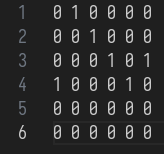
\includegraphics[scale=0.7]{graphs/adj_matrix.png}
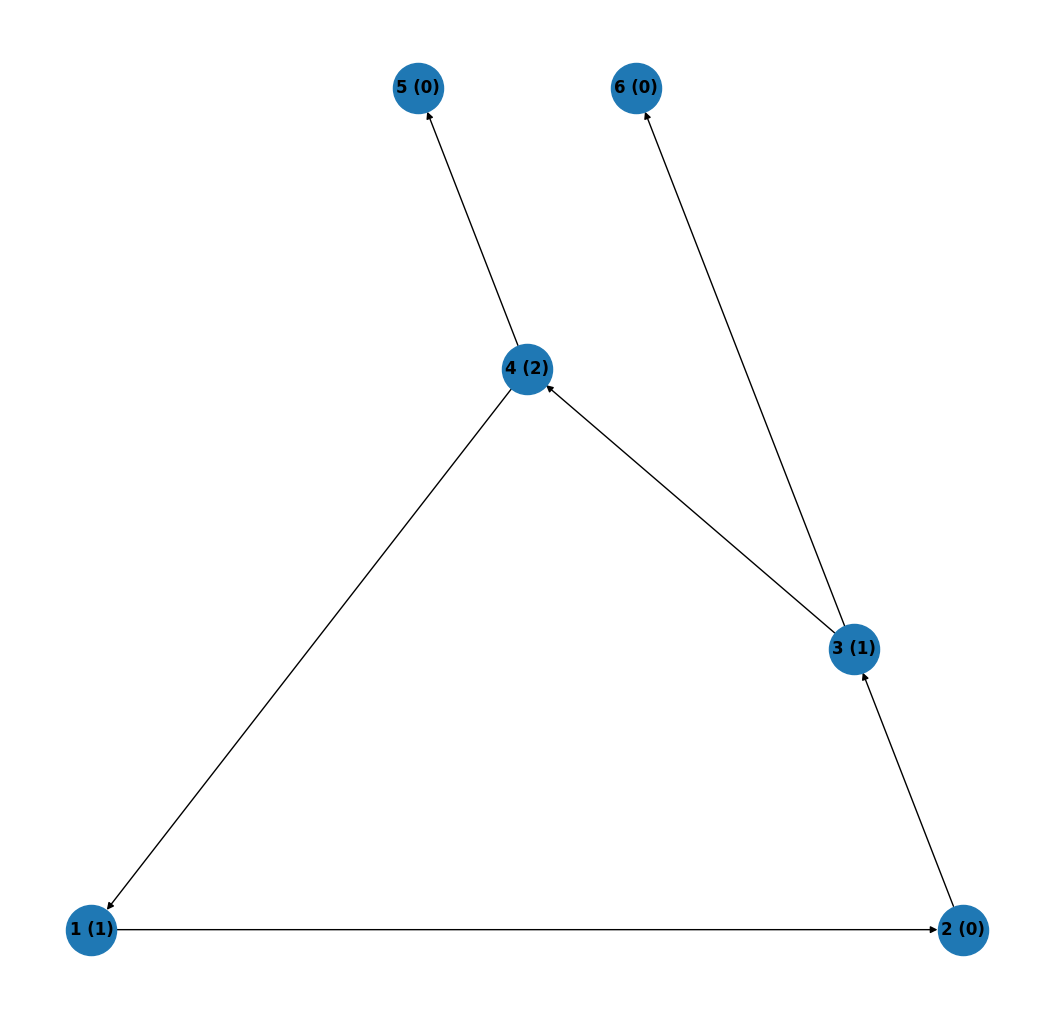
\includegraphics[scale=0.5]{graphs/grundy.png}
\section{Оценка сложности}
Для графа без контуров с количством вершин равным $n$ алгоритм работает за $O(n^3)$,
а для графа с контурами --- за $O(2^n)$ (нахождение ядер графа --- NP-полная задача, поэтому переборный алгоритм является разумным решением).
\section{Прикладная задача}
Функция Гранди позволяет находить выигрышные и проигрышные позиции в игре "\textbf{Фишка на графе}".

\emph{Правила игры}. Дан ориентированный ациклический граф. В некоторой его вершине находится фишка. Играют двое, ходы делаются по очереди. За один ход можно переместить фишку в любую вершину, в которую существует ребро из текущей. Проигрывает тот, кто не может сделать следующий ход.
Как и ранее, при анализе данной игры можно отметить выигрышные и проигрышные вершины.

При этом можно использовать такие соображения:
\begin{itemize}
    \item начать можно с того, что вершины, из которых не выходит ни одного ребра, будут проигрышными (то есть, если перед ходом какого-то игрока фишка стоит в такой вершине, то он проиграл, так как не сможет сделать ход)
    \item любая вершина, из которой есть хотя бы одно ребро, ведущее в проигрышную — будет выигрышной;
    \item любая вершина, из которой можно попасть только в выигрышные — сама является проигрышной.
\end{itemize}

Так как в перспективе мы собираемся рассмотреть сумму из таких игр, то в данной задаче будем не просто выяснять является ли вершина выигрышной или проигрышной, а для каждой вершины будем вычислять функцию Гранди

Функция Гранди равна нулю для всех проигрышных вершин и положительна для всех выигрышных.

Для того, чтобы ответить на вопрос «кто выиграет?» достаточно вычислить функцию для той вершины, где в начальный момент находится фишка.

Чтобы ответить на вопрос: «какой ход нужно сделать из определенной позиции?» нужно рассмотреть все исходящие ребра для текущей вершины. Если вершина является выигрышной, то, по построению, из нее обязательно будет хотя бы один ход в одну из проигрышных. Этот ход и нужно делать.

Усложним задачу: \textbf{много фишек на графе}.

\emph{Правила игры}. Дан ориентированный ациклический граф. В некоторых его вершинах находятся фишки. Играют двое, ходы делаются по очереди. За один ход можно переместить фишку в любую вершину, в которую существует ребро из текущей. Проигрывает тот, кто не может сделать следующий ход. В процессе игры разрешается размещать несколько фишек в одной вершине.

Эта игра является суммой нескольких предыдущих игр.
То есть, ее можно рассматривать как несколько одновременно происходящих игр, каждая из которых ведется с единственной фишкой. В этом случае перед игроком появляется дополнительная задача.

Во-первых, следует правильно выбрать в какой из элементарных игр он будет делать ход (какую фишку он будет двигать). При этом данная элементарная игра не должна быть завершена (ход этой фишкой должен быть возможен).

Во-вторых, следует сделать правильный ход выбранной фишкой.

Для этого мы будем использовать функцию Гранди $g$.
\begin{itemize}
    \item Вычислим $g(v)$ для всех вершин графа;
    \item Рассмотрим все вершины, в которых находятся фишки. Тогда общим значением $S$ для суммарной позиции будет  $S = g(v_1) \oplus g(v_2) \oplus \dots \oplus g(v_k)$, где $v_1, \dots, v_k$ –- вершины, в которых стоят фишки, $\oplus$ - побитовое исключающее "или".
\end{itemize}


Если вычисленное значение $S = 0$, то позиция по сумме игр — проигрышная (что не означает проигрыша во всех играх суммы. В отдельных играх суммы возможен выигрыш).

Если вычисленное значение $S > 0$, то позиция по сумме игр — выигрышная (что, опять же, не означает выигрыша во всех играх суммы. В отдельных играх возможен проигрыш).

Правильным будет ход, который приведет к позиции с $S = 0$ (то есть после которого сопернику достанется проигрышная позиция).

\textbf{Пример}

В качестве примера будем использовать граф, для которого уже вычислены значения функции Гранди, они указаны в скобках. Установим несколько фишек, их расположение показано черным цветом.

\begin{figure}[H]\centering\includesvg[scale=0.5]{graphs/game}\caption{Граф с фишками}\end{figure}

Для оценки позиции по сумме игр нужно найти:
$g(v_2) \oplus g(v_5) \oplus F(v_3) = 1 \oplus 3 \oplus 1 = 3$

В приведенном примере необходимо сделать ход фишкой из вершины $v_5$ в вершину $v_6$. Таким образом $g(v_2) \oplus g(v_6) \oplus g(v_3) = 1 \oplus 0 \oplus 1 = 0$.
\end{document}
